% !TEX spellcheck = en_US
% !TeX root = Lecture.tex
%---------------------------------------------------------------------------------
\section[Blade Design]{Blade Design According to Betz}\label{sec:DES}
%---------------------------------------------------------------------------------
\miniframesoff
\begin{frame}<handout:0>[noframenumbering]{Content}
\tableofcontents[currentsection]
\PutAt<1-|handout:0>[5cm]{(10cm,2cm)}{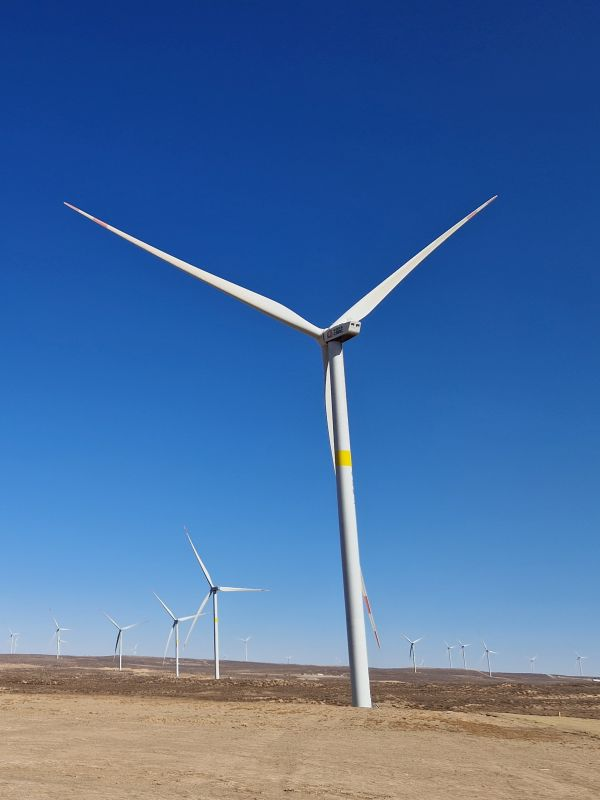
\includegraphics[width=4.0cm]{\StylePath/content/Gobi}} % graphic related to topic	
\end{frame}
\miniframeson
%---------------------------------------------------------------------------------
%%---------------------------------------------------------------------------------
\begin{frame}{Blade Design According to Betz - Main Idea}
\begin{columns}	
	\column{10cm}
	\begin{block}<1->{Inputs}
		\begin{itemize}
			\item Design tip speed ratio $\lambda_{\textnormal{D}}$
			\item Rotor radius $R$			
			\item Number of blades $z$
			\item Design values from airfoils: 
			\begin{itemize}
				\item Angle of attack $\alpha_{\textnormal{A}}$ 
				\item Lift coefficient $c_{\textnormal{L}}$
			\end{itemize}				
		\end{itemize}		
	\end{block}	
	\begin{block}<2->{Outputs}
		\begin{itemize}
			\item Distribution of twist angle $\beta(r)$ over radius
			\item Distribution of chord length $c(r)$ over radius		
		\end{itemize}		
	\end{block}		
	\column{4cm}
	\includegraphics<1->[width=4cm]  {DES/MM92_Rotorblatt}
\end{columns} 	
\end{frame}
%%---------------------------------------------------------------------------------
\begin{frame}[t]{Blade Design According to Betz - Derivation 1/7} 
\setlength{\abovedisplayskip}{0pt}
\setlength{\belowdisplayskip}{0pt}
\vspace*{-0.2cm} %compensate [t]
\begin{columns}[T]	
	\column{6cm}
	\begin{block}<1->{Triangle of velocities}
		\begin{align*}		
			\tan{\left( \phi(r) \right)}&=\frac{v_2}{u(r)}=\frac{2 v_1}{3 \Omega r}\\
			\lambda_{\textnormal{D}}& =\frac{\Omega R}{v_1} 
		\end{align*}		
	\end{block}	
	\begin{block}<2->{Distribution twist angle}
		\begin{align*}		
			\beta(r)   & = \phi(r)-\alpha_{\textnormal{A}}\\
			& = \arctan\left( \frac{2}{3} \frac{R}{r\lambda_{\textnormal{D}}}\right)-\alpha_{\textnormal{A}}
		\end{align*}		
	\end{block}	
	\column{8cm}
	\includegraphics<1->[width=8cm] {DES/Twist.pdf}
\end{columns} 	
\begin{block}<3>{Blade design according to Betz}
	We now have already the first output (twist angle) only depending on the inputs $R$, $\lambda_{\textnormal{D}}$, $\alpha_{\textnormal{A}}$! 
\end{block}	
\end{frame}
%%---------------------------------------------------------------------------------
\begin{frame}[t]{Blade Design According to Betz - Derivation 2/7}
\vspace*{-0.2cm} %compensate [t]
\begin{columns}[T]	
	\column{6cm}
	\begin{block}<1->{Strategy to get the chord length}
		\begin{enumerate}
			\item Get the tangential force on each blade section.
			\item Use the tangential force to calculate the mechanical power for each blade section neglecting the drag.
			\item Set the mechanical power equal to the maximum power.
			\item Use the triangle of velocity at a blade section to get the chord length only depending on inputs.
		\end{enumerate}	
	\end{block}	
	\column{8cm}
	\includegraphics<1->[width=8cm] {DES/Chord}
\end{columns} 		
\end{frame}
%---------------------------------------------------------------------------------
\begin{frame}[t]{Blade Design According to Betz - Derivation 3/7} 
\setlength{\abovedisplayskip}{0pt}
\setlength{\belowdisplayskip}{0pt}
\vspace*{-0.2cm} %compensate [t]
\begin{columns}[T]	
	\column{6cm}
	\begin{block}<1->{Lift force and drag force}
		\begin{align*}
			\textnormal{d}L   & = \frac{1}{2} \rho \left(c\textnormal{d}r\right) c_{\textnormal{L}}w^2\\
			\textnormal{d}D   & = \frac{1}{2} \rho \left(c\textnormal{d}r\right) c_{\textnormal{D}}w^2
		\end{align*}
		\begin{tabular}{ll}
			$\textnormal{d}r$ 		&	chord width at section $r$ 
		\end{tabular}	
	\end{block}
	\begin{block}<2->{Tangential force and thrust force}
		\begin{align}
			\textnormal{d}U   	& = \textnormal{d}U_L - \textnormal{d}U_D 				\nonumber\\
							 	& = \sin(\phi)\textnormal{d}L-\cos(\phi)\textnormal{d}D \label{equ:DES:U}\\
			\textnormal{d}T   	& = \textnormal{d}T_L+\textnormal{d}T_D 				\nonumber\\
								& = \cos(\phi)\textnormal{d}L+\sin(\phi)\textnormal{d}D \nonumber
		\end{align}	
	\end{block}
	\column{8cm}
		\only<1|handout:0>{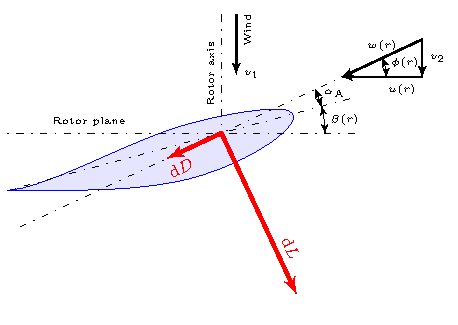
\includegraphics[width=8cm] {DES/Triangle1.pdf}}%
		\only<2|handout:0>{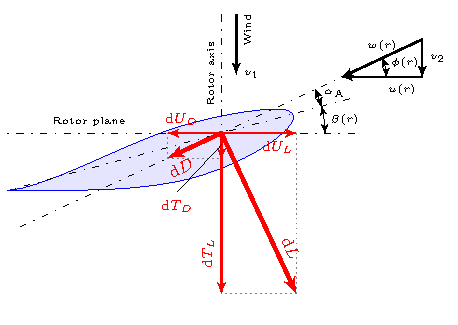
\includegraphics[width=8cm] {DES/Triangle2.pdf}}%
		\only<3|handout:1>{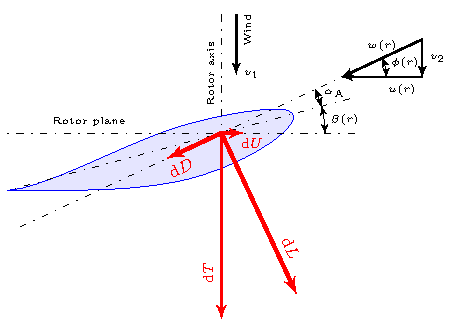
\includegraphics[width=8cm] {DES/Triangle3.pdf}}%
\end{columns}	
\end{frame}
%%---------------------------------------------------------------------------------
\begin{frame}{Blade Design According to Betz - Derivation 4/7} 
\setlength{\abovedisplayskip}{0pt}
\setlength{\belowdisplayskip}{0pt}
\begin{columns}	
	\column{9cm}
	\begin{block}<1->{Mechanical power for each ring section}
	\begin{align}
	\textnormal{d}P_{\textnormal{mech}} 	
		& = z \textnormal{d}U r \Omega \quad\textnormal{with}\quad c_{\textnormal{D}} \ll c_{\textnormal{L}} \quad\textnormal{and}\quad (\ref{equ:DES:U}) \nonumber\\
		& = z   \sin(\phi) \frac{1}{2} \rho \left(c\textnormal{d}r\right)w^2 c_{\textnormal{L}} r \Omega \label{equ:DES:dP}
	\end{align}
	\begin{tabular}{ll}
		$z$ 		& number of blades
	\end{tabular}			
	\end{block}	
	\begin{block}<2->{Maximum power over rotor area}
	\begin{align*}
		P_{\textnormal{Betz}}   & = \frac{16}{27} \frac{\rho}{2}  Av_1^3
	\end{align*}		
	\end{block}	
	\begin{block}<3->{Maximum power for each ring section $\textnormal{d}A=2\pi r \textnormal{d}r$}
		\begin{align}
			\textnormal{d}P_{\textnormal{Betz}}   & = \frac{16}{27} \frac{\rho}{2} (2\pi r \textnormal{d}r) v_1^3\label{equ:DES:dPBetz}
		\end{align}		
	\end{block}	
	\column{5cm}
	\includegraphics<1->[width=5cm] {DES/RingSection}\\% ersetzen durch Tikz aus IWTA#06
	\flushright\tiny\textcolor{gray}{\cite{Gasch2012a}}
\end{columns} 	
\end{frame}
%%---------------------------------------------------------------------------------
\begin{frame}{Blade Design According to Betz - Derivation 5/7} 
	\begin{block}<1->{}
		Setting (\ref{equ:DES:dPBetz}) equal (\ref{equ:DES:dP}) yields
		\begin{align*}
			\frac{16}{27} \frac{\rho}{2} \left( 2\pi r \textnormal{d}r \right) v_1^3 & = z \sin{(\phi)} \frac{1}{2} \rho ( c \textnormal{d} r ) w^2 c_{\textnormal{L}} r \Omega 
		\end{align*}		
	\end{block}		
	\begin{block}<2->{}
		Simplifying yields
		\begin{align*}			
			\frac{16}{27} \frac{\cancel{\rho}}{\cancel{2}} \left( 2\pi \cancel{r} \cancel{\textnormal{d}r} \right) v_1^3 & = z \sin{(\phi)} \frac{1}{\cancel{2}} \cancel{\rho} ( c \cancel{\textnormal{d}r} ) w^2 c_{\textnormal{L}}\cancel{r} \Omega \\
			\frac{16}{27}  \left( 2\pi \right) v_1^3 & = z \sin{(\phi)}  c   w^2 c_{\textnormal{L}} \Omega
		\end{align*}			
	\end{block}	
	\begin{block}<3->{}
		Rearranging yields (chord length still depending on $v_1$, $w$, $\Omega$, and $\phi$ and not on inputs only!)
		\begin{align}			
			c   & = \frac{1}{z} \frac{16}{27} \frac{2\pi}{c_{\textnormal{L}}} \frac{v_1^3}{\Omega w^2 \sin(\phi)} \label{equ:DES:c}
		\end{align}			
	\end{block}	
\end{frame}
%%---------------------------------------------------------------------------------
\begin{frame}[t]{Blade Design According to Betz - Derivation 6/7} 
\setlength{\abovedisplayskip}{0pt}
\setlength{\belowdisplayskip}{0pt}
\vspace*{-0.2cm} %compensate [t]
\begin{columns}[T]	
	\column{6cm}	
	\begin{block}<1->{Term to replace}
		\begin{align*}			
		\frac{v_1^3}{\Omega w^2 \sin(\phi)}
		\end{align*}			
	\end{block}	
	\begin{block}<2->{Triangle of velocities}
		\begin{align}	
		\Omega & = \frac{\lambda_{\textnormal{D}} v_1}{R}\label{equ:DES:Omega}\\
		w \sin{(\phi)}& = \frac{2}{3} v_1\label{equ:DES:sin}
		\end{align}	
	\end{block}	
	\column{8cm}
	\includegraphics<1->[width=8cm] {DES/Twist.pdf}
\end{columns}
\vspace*{-.5cm} 	
	\begin{block}<3->{}	
		\begin{align}
		w^2 &= \left( \frac{2}{3}v_1 \right)^2 + \left( \Omega r \right)^2 = \frac{4}{9}v_1^2+ \left( \frac{\lambda_{\textnormal{D}}v_1}{R} \right)^2 r^2 \quad \Rightarrow \quad w=v_1 \sqrt{\left( \frac{r}{R}\lambda_{\textnormal{D}} \right)^2 + \frac{4}{9}}\label{equ:DES:w}
		\end{align}
	\end{block}	
\end{frame}
%%---------------------------------------------------------------------------------
\begin{frame}{Blade Design According to Betz - Derivation 7/7} 
	\setlength{\abovedisplayskip}{0pt}
	\setlength{\belowdisplayskip}{0pt}
	\begin{block}<1->{}
		Inserting (\ref{equ:DES:Omega},\ref{equ:DES:sin},\ref{equ:DES:w})  in (\ref{equ:DES:c}):
		\begin{align*}
		    c(r) 	&  = \frac{1}{z} \frac{16}{27} \frac{2\pi}{c_{\textnormal{L}}} \frac{v_1^3}{\Omega w^2 \sin(\phi)}\\
		    		&  = \frac{1}{z} \frac{16}{27} \frac{2\pi}{c_{\textnormal{L}}} \frac{v_1^3}{\frac{\lambda_{\textnormal{D}} v_1}{R} \frac{2}{3}v_1 v_1 \sqrt{\left( \frac{r}{R}\lambda_{\textnormal{D}} \right)^2 + \frac{4}{9}}}
		\end{align*}
	\end{block}
	\begin{block}<2->{Distribution chord length}
		\begin{align*}
		c(r) & = \frac{1}{z} \frac{8}{9} \frac{2\pi R}{c_{\textnormal{L}}} \frac{1}{ \lambda_{\textnormal{D}} \sqrt{\left(\lambda_{\textnormal{D}}\frac{r}{R} \right)^2+\frac{4}{9}}} 
		\end{align*}
	\end{block}
	\begin{block}<3>{Blade design according to Betz}
		We finally have the second output (chord length) only depending on the inputs $z$, $R$, $\lambda_{\textnormal{D}}$, $c_{\textnormal{L}}$! 
	\end{block}	
\end{frame}
%%---------------------------------------------------------------------------------
\begin{frame}{Influence of design tip speed ratio $\lambda_{\textnormal{D}}$} 
\begin{columns}
    \column{7cm}
    \includegraphics<1->[width=7cm] {DES/Gasch2012_Fig5.16.pdf}\\
    \tiny\textcolor{gray}{\cite{Gasch2012a}}
    \column{7cm}
	\includegraphics<1->[width=7cm] {DES/Hau2006_Fig5.30.jpg}\\
	\flushright\tiny\textcolor{gray}{\cite{Hau2006}}
\end{columns}
\end{frame}
%---------------------------------------------------------------------------------
\begin{frame}{Solidity} 
\centering
\includegraphics<1->[height=7cm] {DES/Gasch2012_Fig5.15.pdf}\\
\tiny\textcolor{gray}{\cite{Gasch2012a}}
\end{frame}
%%---------------------------------------------------------------------------------
\begin{frame}{Remark: Real Turbines don't reach the Betz limit} 
\centering
	\begin{block}<1->{}	
	\begin{itemize}
		\item maximum power coefficient according to Betz $16/27\approx 59\%$ 		
		\item real power coefficient usually around  $43\%-48\%$ 
		\item Enercon E66 with E4-Blade reaches $52\%$ 
	\end{itemize}	
	\end{block}
\includegraphics<1->[width=5.5cm] {DES/Enercon1}
\includegraphics<1->[width=5.5cm] {DES/Enercon2}
\tiny\textcolor{gray}{[Enercon]}
\end{frame}
%---------------------------------------------------------------------------------
\begin{frame}{Some impressions from the Original Work by Betz 1/3} 
\begin{columns}	
	\column{7cm}
		\centering
		\includegraphics<1->[height=7.5cm] {DES/Betz1926_Frontpage}{\tiny\textcolor{gray}{\cite{Betz1926}}}
	\column{7cm}
		\centering
		\includegraphics<2->[height=7.5cm] {DES/Betz1926_Abb7}{\tiny\textcolor{gray}{\cite{Betz1926}}}
\end{columns} 
\end{frame}
%---------------------------------------------------------------------------------
\begin{frame}{Some impressions from the Original Work by Betz 2/3} 
	\centering
	\includegraphics<1->[height=7.5cm] {DES/Betz1926_Page12and13}
	{\tiny\textcolor{gray}{\cite{Betz1926}}}
\end{frame}
%---------------------------------------------------------------------------------
\begin{frame}{Some impressions from the Original Work by Betz 3/3} 
\centering
\includegraphics<1->[height=7.5cm] {DES/Betz1926_Page24and25}
{\tiny\textcolor{gray}{\cite{Betz1926}}}
\end{frame}
%---------------------------------------------------------------------------------
\begin{frame}{Outlook: Real blades look different} 
\centering
\includegraphics<1->[width=6.5cm] {DES/Gasch2012_Fig3.9.jpg}{\tiny\textcolor{gray}{\cite{Gasch2012a}}}
\includegraphics<1->[width=6.5cm] {DES/MM92_blade.jpg}
\end{frame}
%%---------------------------------------------------------------------------------
\begin{frame}{Outlook: Blade Design According to Schmitz} 
\begin{columns}
	\column{7cm}
	\begin{block}<1->{Considered real effects}	
		\begin{itemize}
			\item Wake losses
			\item Airfoil drag
			\item Finite number of blades
		\end{itemize}	
	\end{block}
	\includegraphics<1->[height=4.5cm] {DES/Hau2006_Fig5.7.jpg}\\
	\flushright\tiny\textcolor{gray}{\cite{Hau2006}}	
	\column{7cm}
	\begin{block}<2->{Comparison for chord length}	
		\begin{itemize}
			\item Similar for large $\lambda_{\textnormal{D}}$ and close to tip
			\item Different for small $\lambda_{\textnormal{D}}$ and close to hub
		\end{itemize}	
	\end{block}%
	\includegraphics<2->[width=7.0cm] {DES/Gasch2012_Fig5.22}%
	\visible<2->{\flushright{\tiny\textcolor{gray}{\cite{Gasch2012a}}}}%
\end{columns} 
\end{frame}
%%---------------------------------------------------------------------------------